\chapter{Unavailable Time/Preferred Teaching Time}
\label{zeitsperren_zeitwuensche}

\section{General}

The preferred teaching times and unavailable times can be found under "My CIS".
They primarily serve to support the planning of the teaching schedule to display availability and schedule preferences there.
The vacations booked in the vacation tool (see chapter \ref{urlaubsverwaltung}) are also saved in the system as unavailable times and can as such be edited there as well.

\section{Unavailable Time}
\label{zeitsperren}

In contrast to the preferred teaching time, the unavailable time is intended for marking specific times as unavailable.
An unavailable time is marked with an exact date (from - to) and time (from - to) and can also be provided with additional optional information (e.g. reason for unavailability, substitute,...).

Unavailable time is to be used for example for compensatory time, conferences, sick leave, business travel and other similar events (see Fig. \ref{eingabemaske_zeitsperren}).

\begin{itemize}
	\item Select a "'reason"' for being unavailable from the drop-down menu and enter a meaningful name for the unavailable time.
	\item Please enter the dates and optionally the units for which you will not be available in the "'From"' and "'To"' fields.
	\item Next to "'accessibility"' you can select whether can be reached by telephone, email or if you can not be reached at all while you are away.
	\item Finally, you can also specify someone as your substitute.
	\item Clicking the "'Add"' button confirms and saves your unavailable time.	
\end{itemize}

Selecting "'vacation"' as the reason for your unavailable time is the same as booking a vacation using the vacation tool (see chapter \ref{urlaubsverwaltung}).
For this reason, the unavailable time is processed the same way as booking a vacation, with an email being sent to your manager for approval. Such unavailable times will also be deducted from your accrued vacation.

\achtung{All the days entered will be considered vacation days when calculating your accrued vacation! Therefore, it is necessary to divide longer unavailable times marked as vacation so that they do not include weekends or holidays!}


\begin{figure}
	\centering
	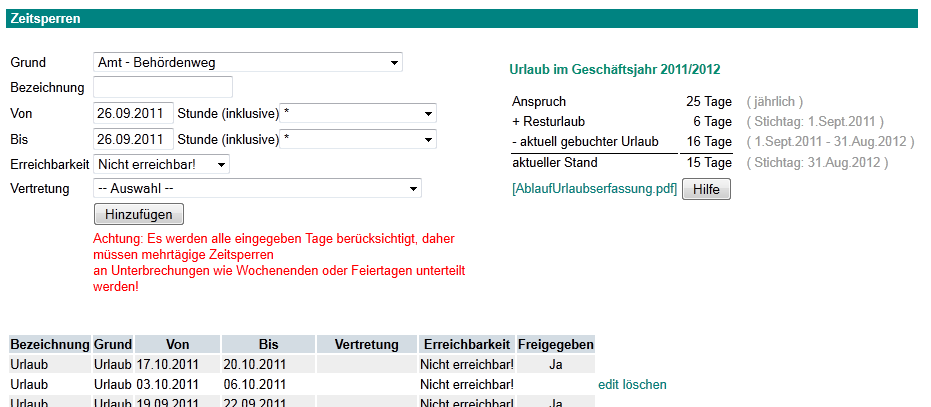
\includegraphics[width=0.70\textwidth]{CIS_Zeitsperre.png}
	\caption{User Interface for Unavailable Times}
	\label{eingabemaske_zeitsperren}
\end{figure}

\subsection{Editing/Deleting Unavailable Times}

The unavailable times you have entered appear in a list below the form.
Next to each entry (excluding approved vacations) you will see an "'Edit"' and a "'Delete"' button which you can use to edit or delete the entry.

You can not edit or delete approved vacations. If you wish to edit or delete an approved vacation, please contact your manager.

\section{Preferred Teaching Time}

The preferred teaching time is entered only once in a static standard weekly grid and is intended to provide a rough template for the availability of the lecturers during a "'normal"' week.

The lecturer can assign values from -2 to +2 for every day and every unit in a week to indicate their availability.
Based on the preferred teaching time, the planning of the teaching schedule can take into account the times a lecturer would like to teach.

The preferred teaching time should and can NOT represent exact availability, but should only serve as a means of orientation.
In order to provide a more detailed overview of availability, please use the unavailable time feature (chapter \ref{zeitsperren}).

\begin{figure}
	\centering
	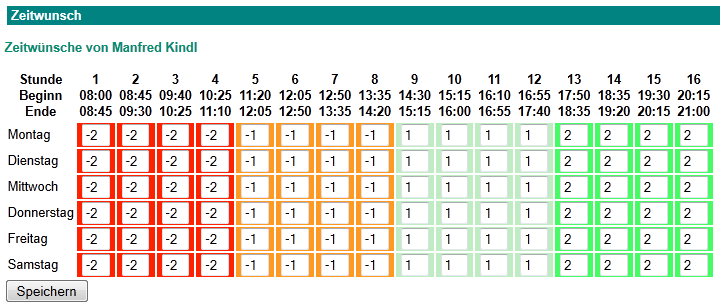
\includegraphics[width=0.70\textwidth]{CIS_Zeitwunsch.png}
	\caption{Preferred Teaching Time Entry Form}
\end{figure}

The default value for the preferred teaching time is "'+1"' for all units.

Now enter the desired value (-2 to +2) in each unit that you want to change and confirm your preferred teaching time by clicking on "'Save"'.

\begin{tabular}{rll}
+2&...&I would like to teach at this time\\
+1&...&I can teach at this time\\
-1&...&I would prefer not to teach at this time\\
-2&...&I can not at all teach at this time\\
\end{tabular}

\idee{You can quickly move between cells by pressing the tab key on your keyboard.}

The values are shown in the background according to a color system (from red to green).
 
Please note the following:

\begin{enumerate}
	\item To make a better optimization possible, please only use the value of -2 if you really can not teach at this time.
	\item The preferred teaching times should be chosen according to the fair play principle, so that at least three times as many teaching units are assigned a positive value as are to be taught according to the teaching assignment. \\ Example: If you are teaching 4 hours/week, then you should select at least 12 hours of preferred teaching times in the grid. 
\end{enumerate}